\documentclass[conference]{IEEEtran}
\IEEEoverridecommandlockouts
% The preceding line is only needed to identify funding in the first footnote. If that is unneeded, please comment it out.
\usepackage{cite}
\usepackage{amsmath,amssymb,amsfonts}
\usepackage{algorithmic}
\usepackage{graphicx}
\usepackage{textcomp}
\usepackage{xcolor}
\def\BibTeX{{\rm B\kern-.05em{\sc i\kern-.025em b}\kern-.08em
    T\kern-.1667em\lower.7ex\hbox{E}\kern-.125emX}}
\begin{document}

\title{Different Types of loop in C}

\author{\IEEEauthorblockN{Rupa Nayak}
\IEEEauthorblockA{\textit{Maste of Computer Application} \\
\textit{Kalyani Government Eng. College}\\
Kalyani,Nadia,India \\
rupa.nayak98@gmail.com}
}

\maketitle

\begin{abstract}
Besides all other programming languages C also have the special feature to execute block of statements more than one time, which is called 'Loop'. This loops helps C programs more structured and more effective. There exist different types of loops in C. Let's learn about then for writing better C programs.
\end{abstract}

\section{INTRODUCTION}
C is a middle level structured programming language because it have a very special feature such as different types of Loops. Loop controls structures are used when we want to execute a block of statements several times. Loop statement always comes with a conditional statement. Until the condition become ‘false’ the loop will execute continuously. There are three types of loop control statements in C programming language

\begin{itemize}
  \item \textbf{for loop
  \item while loop
  \item do-while loop}
\end{itemize}


\section{Detail explanations are given below-}
\subsection{for loop}
The ‘for’ loop statement is very useful to write programs in C language. It has three expressions in ‘for’ loop separated by semicolons (;). The ‘for’ loop statements are written as-
\linebreak
\linebreak
\hspace*{1cm}for(expression1;expression2;expression3){
\linebreak
\hspace*{2cm}statement1;
\linebreak
\hspace*{2cm}statement2;
\linebreak
………………….
\linebreak
\}
\linebreak
\linebreak

The body of the loop can be single statement or a block of statement. If the body contains only one statement the it can be written as-
\linebreak
\linebreak
\hspace*{1cm}for(expression1;expression2;expression3)
\hspace*{2cm}statement;
\linebreak
\linebreak
\linebreak
Here expression1 is the initialisation expression, expression2 is conditional expression and expression3 is an update expression. Expression1 is first executed when the loop is started and this expression initialised the loop variable. This expression executes only ones. Then expression2 is condition and is tested before each iteration of the loop. This expression generally relational and logical operator. When this expression becomes false the loop terminated. Expression3 is used to update the loop variable after each iteration. This expression generally increment or decrement operator.

First expression1 is executed and initialised the loop variable. Then the compiler check the expression2, either the given condition become false or not. If the condition become false the loop terminated and executing following statements after the ‘for’ loop closing brush. If the condition become true then body of the loop is executed and the control is shifted to the expression3 statement of the ‘for’ loop. The expression3 update loop variable and again control transfer to expression2 for checking the condition to be true or false .In this repeated way the loop is executed. Flow chart is given below for better understanding-

\begin{figure}[h!]
\centering
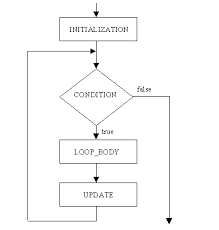
\includegraphics[width=70mm]{for.png}
\caption{Flow chart of "for" loop}
\label{fig:method}
\end{figure}

	This loop is generally used when the number of iterations are known in advance. Let’s see an example using ‘for’ loop. Suppose we want to print the sum of first 10 numbers.
\linebreak
\linebreak
\hspace*{1cm}for(i=1;i<=10;i++)\{
\linebreak
\hspace*{2cm}s=s+i;
\linebreak
\hspace*{3cm}\}
\linebreak
Here in the starting of the loop the loop variable ‘i’ is initialised by 1 and the check whether ‘i’ is equal to 10 or not. ‘i’ is not 0, so the value of ‘i’ is added with and then the value of ‘i’ is incremented by 1. Again the control checks the condition and so on. When the value of ‘i’ becomes 10 then loop will terminated and started execute the rest of the program.

\subsection{while loop}

 While loop is also a very popular loop. This loop is generally used when the no of iterations do not know in advance. 
‘while’ loop is represented as-
\linebreak
\linebreak
\hspace*{1cm}While(expression){
\linebreak
\hspace*{2cm}Statement1;
\linebreak
\hspace*{2cm}Statement2;
\linebreak
\hspace*{2cm}\}
\linebreak
\linebreak
If there exist only one statement in the body of the loop then the loop can be written as
\linebreak
\linebreak
\hspace*{1cm}While(expression)
\linebreak
\hspace*{2cm}Statement;
\linebreak
\linebreak
This loop first check whether the loop variable satisfy the condition or not. If loop variable satisfy the condition the body of the loop will be executed and go to next iteration and check the condition again. If the condition becomes false the loop will be terminated.
For this featured of ‘while’ loop it is called as ‘entry control’ loop.  
The flow chart of ‘while’ loop is given below-
\linebreak
\linebreak
\begin{figure}[h!]
\centering
\includegraphics[width=70mm]{while.jpg}
\caption{Flow Chart of while loop}
\label{fig:method}
\end{figure}
Suppose we want to print 1 to 10 numbers using ‘while’ loop-
\linebreak
\linebreak
 a = 1;
\linebreak
while (a<=10){
\linebreak
\hspace*{1cm}printf (“%d “, a);
\linebreak
\hspace*{1cm}a++;
\linebreak
\}
\linebreak
Here loop variable a is initialised before entering the loop and check for condition and the condition is true so the value will be printed and increment the value of a by a. After the body of the loop is finished as well as next iteration will be started and again check the condition and so on.
\linebreak
\subsection{do-while loop}

It is also a loop but do not used frequently. This loop can be represented as –
\linebreak
do{
\linebreak
\hspace*{1cm}Statemebt1;
\linebreak
\hspace*{1cm}Statement2;
\linebreak
\hspace*{1cm}…………….
\linebreak
\}while(expression);
The body of the loop can contain one or more sentences. In this loop first body of the loop is executed and at the end of each iteration condition has been checked. For this reason it is called ‘exit control’ loop. It is basically used in menu driven programs.
\linebreak
Flow chart of ‘do-while’ loop is as follow-
\begin{figure}[h!]
\centering
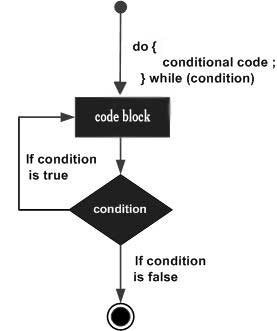
\includegraphics[width=70mm]{do.jpg}
\caption{Flow Chart of do while loop}
\label{fig:method}
\end{figure}
Here firstly body of the loop is executed then condition is evaluated. If the condition is true the body of the loop is executed repeatedly until the condition become false. In this loop the semicolon (;) is placed after the condition.
\linebreak
Suppose we want inputs from user until it is 0 and the print it.
\linebreak
do\{
\linebreak
\hspace*{1cm}printf(“Enter a number (0 to stop):  ”);
\linebreak
\hspace*{2cm}scanf(“\%d”,\&n);
\linebreak
\hspace*{1cm}printf(“\%d”,n);
\linebreak
\}while(n);

First the program asked for a number. Then number has been printed and then check if the number is 0 or not. If it is 0 then the loop terminated otherwise again asked for another number and so on.

\end{document}
